\begin{tiny}(Cmo02)\end{tiny} Pour la première matrice, on applique l'algorithme I dans un contexte formel avec un paramètre $m$.
Pour ne pas introduire de cas particulier inutile, $m$ ne doit pas figurer dans les valeurs pivots. On forme la liste des matrices transformées
\begin{multline*}
  \begin{pmatrix}
    m & -1 & 0 \\
    -2 & m & -2 \\
    0 & -1 & m
  \end{pmatrix}
\rightarrow
  \begin{pmatrix}
    -2 & m & -2 \\
    m & -1 & 0 \\
    0 & -1 & m
  \end{pmatrix} \\
\rightarrow
  \begin{pmatrix}
    -2 & m & -2 \\
    0 & -1 + \frac{m^2}{2} & -m \\
    0 & -1 & m
  \end{pmatrix} \\
\rightarrow
  \begin{pmatrix}
    -2 & m & -2 \\
    0 & -1 & m\\
    0 & -1 + \frac{m^2}{2} & -m 
  \end{pmatrix}
\rightarrow
  \begin{pmatrix}
    -2 & m & -2 \\
    0 & -1 & m\\
    0 & 0 & P(m) 
  \end{pmatrix} \\
\text{ avec }
P(m) = -m + \left( -1 + \frac{m^2}{2}\right)m
= \frac{1}{2}m(m^2 - 4).
\end{multline*}

Le rang est 3 sauf si $m\in \left\lbrace -2, 0, 2\right\rbrace$.\newline
Si $m = -2$ la matrice est équivalente à
\[
  \begin{pmatrix}
    -2 & -2 & -2 \\
    0 & -1 & -2\\
    0 & 0 & 0 
  \end{pmatrix}
  \text{ de rang 2.}
\]
Dans les deux autres cas, les deux premières colonnes forment une famille libre le rang est encore 2.

Pour la deuxième matrice, on fait des opérations élémentaires qui conservent le rang 
\begin{multline*}
\begin{pmatrix}
  2+a+b &  a & 1 & b \\
  2+a+b &  1 & b & 1 \\
  2+a+b &  b & 1 & a \\
  2+a+b &  1 & a & 1
\end{pmatrix} C_1 \leftarrow C_1 + C_2 + C_3 + C_4\\
\rightarrow
\begin{pmatrix}
  2+a+b &  a  & 1   & b   \\
  0     & 1-a & b-1 & 1-b \\
  0     & b-a & 0   & a-b \\
  0     & 1-a & a-1 & 1-b
\end{pmatrix} L_i \leftarrow L_i - L_1\\
\rightarrow
\begin{pmatrix}
  2+a+b &  a  & 1   & b   \\
  0     & 1-a & b-1 & 1-b \\
  0     & b-a & 0   & a-b \\
  0     & 0   & a-b & 0
\end{pmatrix} L_4 \leftarrow L_4 - L_2 \\
\rightarrow
\begin{pmatrix}
  2+a+b & a+b   & 1   & b   \\
  0     & 2-a-b & b-1 & 1-b \\
  0     & 0     & 0   & a-b \\
  0     & 0     & a-b & 0
\end{pmatrix} \\ C_2 \leftarrow C_2 + C_4 \\
\rightarrow
\begin{pmatrix}
  2+a+b & a+b   & b   & 1   \\
  0     & 2-a-b & 1-b & b-1 \\
  0     & 0     & a-b & 0 \\
  0     & 0     & 0 & a-b
\end{pmatrix} \\ C_2 \leftrightarrow C_3
\end{multline*}

Sous cette forme il est clair que le rang est 4 sauf si une ou plusieurs des conditions suivantes sont vérifiées
\[
  \left\lbrace
  \begin{aligned}
    2+a+b &= 0 \\ 2-a-b &= 0 \\ a-b &= 0
  \end{aligned}
  \right.
\]
Ces conditions traduisent dans le plan $\R^2$ l'appartenance du point $(a,b)$ à certaine droites.
\begin{figure}[h!]
  \centering
  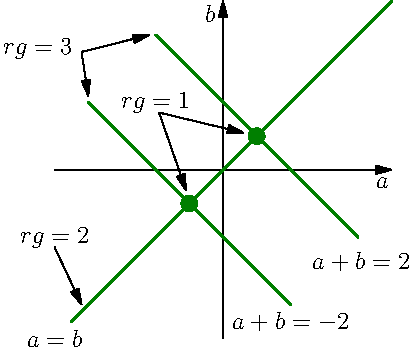
\includegraphics[width=5cm]{Cmo02_1.pdf}
  % Cmo02_1.pdf: 79x85 px, 72dpi, 2.79x3.00 cm, bb=0 0 79 85
  \caption{Ex \ref{num_Emo02} (Emo02) Rangs dans $\R^2$.}
\end{figure}
